\section{Experimental Evaluation} \label{sec:experiments}

This section presents the research questions and the experiments we conducted and analyzed to validate our approximate distributed monitoring approach.

\subsection{Research Questions}

We seek answers to the following research questions (RQs):

\begin{resq}[What is the tradeoff between the efficiency and the accuracy of approximate distributed monitors?]
The  approximate distributed monitoring comes with a price in terms of the loss of accuracy.
We want to understand the tradeoff between the potential speed-ups that an approximate distributed monitor can achieve when compared to its exact counterpart and the consequent loss in accuracy due to the approximations.
We would also like to identify the classes of signals and properties for which this tradeoff is effective. 
\end{resq}

\begin{resq}[Can the combination of approximate and exact distributed monitors increase efficiency while preserving accuracy?]
We are interested in evaluating whether a smart, combined use of approximate and exact distributed monitors can still bring improvements in monitoring efficiency while guaranteeing the accuracy of the monitoring verdicts. 
\end{resq}

\subsection{Experimental Setup}

\subsubsection{Distributed Monitors} \label{sec:testGeneration}
In our study, we compare our approximate distributed monitoring (ADM) approach to a an exact distributed monitoring approach.
For the exact monitoring, we take a variant of the distributed monitoring procedure from~\cite{MomtazAB23} that allows to evaluate STL specifications over distributed traces using SMT-solving.
Originally, that procedure assumes that input signals are polynomial continuous functions.
We adapt the SMT-based approach to consider input signals as piecewise-constant signals to make a consistent comparison with ADM.
We note that the passage from the polynomial continuous to piecewise-constant input signals reduces the efficiency of the SMT-based monitors.
We also observe that the SMT-based monitors from~\cite{MomtazAB23} can split the input trace into multiple segments and evaluate the specification incrementally, segment-by-segment, allowing early termination of the monitor in some cases.
Since the focus of this paper is purely on the offline monitoring, we also use the exact monitors without their incremental mode.
We use the abbreviation EDM to denote the variant of the exact SMT-based distributed monitors used in this study.


\subsubsection{Experimental Subjects}
To answer our research questions, we use (1) a \emph{random generator} (RG) of distributed traces, (2) a \emph{heat pump} (HP) case study, and (3) a \emph{swarm of drones} (SD) case study.  

\noindent \emph{The random generator (RG)} uses uniform distribution to generate distributed traces, in which the user can control the duration $d$ of the trace, as well as the $\epsilon$ bound on the uncertainty at which the events happen.

\noindent \emph{Heat pump (HP)} model is a SimuLink model of a hybrid high pressure water distribution system consisting of two water tanks. Inlet pipes connect each water tank to an external source, and outlet pipes distribute high pressure water that is regulated by valves.
Each valve is operated by a controller that samples the outflow pressure at 20Hz using its local clock. Our model is a simplified emulation of the Refueling Water Storage Tanks (RWST) module of an Emergency Core Cooling System (ECCS) of a Pressurized Water Reactor Plant~\cite{USNRCPWR}.

\noindent \emph{Swarm of drones (SD)} model is generated using a path planning software, Fly-by-Logic~\cite{PantAM17CCTA}. In this simulation, a swarm of drones were set to perform various reach-avoid missions, while securing objectives likes reaching a goal within a deadline, avoiding obstacles, avoiding collisions, and so on. The path planner finds the most robust trajectory using a temporal logic robustness optimizer. These trajectories are sampled at 20Hz.

\subsubsection{Specifications}

Table~\ref{tab:spec} summarizes the STL specifications that we use to monitor the behavior of our three experimental subjects. Specifications $\varphi_{1-5}$ are applied to the distributed traces created by the random generator and represent different classes and fragments of Boolean-valued temporal formulas. The first specification $\varphi_1$ is an LTL formula in which both the outer temporal operator ($\LTLg$) and the inner Boolean operator ($\wedge$) are conjunctive. The second specification $\varphi_2$ puts instead a disjunction within the scope of the conjunctive temporal $\LTLg$ operator. The third specification $\varphi_3$ is a simple \emph{until} formula. The fourth formula $\varphi_4$ is the common LTL response formula, while $\varphi_5$ adds a bounded real-time response requirement to the previous specification. The specification $\varphi_{HP}$ associated to the heat pump case study is an STL formula in which a sum of signals originating from different agents is compared to a constant. FInally, the specification $\varphi_{SD}$ defines a mutual separation property that requires more sophisticated arithmetic operations on signals originating from different agents.  

\begin{table}
\centering
\begin{tabular}{|l|l|l|l|}
\hline
Subject & Spec ID & STL formula \\
\hline
\multirow{ 5}{*}{RG}
& $\varphi_1$ & $\LTLg (p \wedge q)$  \\
& $\varphi_2$ & $\LTLg (p \vee q)$ & \\
& $\varphi_3$ & $ p \LTLuntil q$ & \\
& $\varphi_4$ & $\LTLg (p \Rightarrow \LTLf q)$ \\
& $\varphi_5$ & $\LTLg (p \Rightarrow \LTLf_{[0,1)} q)$  \\
%& $\varphi_1$ & $\LTLg (p \wedge q)$ & \multirow{ 5}{*}{untimed} \\
%& $\varphi_2$ & $\LTLf (p \vee q)$ & \\
%& $\varphi_3$ & $\LTLg (p \vee q)$ & \\
%& $\varphi_4$ & $\LTLf (p \wedge q)$ & \\
%& $\varphi_5$ & $p \until q$ & \\
\hline
HP & $\varphi_{HP}$ & $\LTLg \left(\sum_{i=1}^{n} x_i  > c\right)$  \\
SD & $\varphi_{SD}$ & $\bigwedge_{1 \leq i \neq j \leq n} \LTLg \left( \sqrt{(x_i-x_j)^2 + (y_i-y_j)^2 + (z_i-z_j)^2} > c \right)$   \\
\hline
\end{tabular}
\caption{STL specifications used in the experiments.}
\label{tab:spec} 
\end{table}

\subsubsection{Computing Platform}

To conduct the experiments, we used a laptop with Ubuntu 24.04, an AMD Ryzen 7 4800HS CPU at 2.90 GHz clock rate, and 16GB of RAM.
Our tool is implemented in C++ and compiled using \texttt{g++} version 13.2.0 with the optimization flag \texttt{-O3} enabled.
The precise method invokes the SMT-solver Z3 \cite{MouraB08} and is based on \cite{MomtazAB23}.

\subsubsection{Results}
\ege{maybe we can move some of the synthetic experiments to the appendix?}

We first conducted the experiments on ditributed traces created by RG and evaluated on specifications $\varphi_1$ to $\varphi_5$. Figure~\ref{fig:rgresults} summarizes the results of the experiments. Each row in Figure~\ref{fig:rgresults} shows the result for a specific formula. The first column in the figure depicts a heatmap where each cell shows how many times ADF is faster than EDF when evaluating the formula on the give distributed trace with duration $d$ and uncertainty bound $\epsilon$. The second column shows a heatmap where every cell shows the percentage of \emph{false postitives} (FP) introduced by ADM, where a false positive happens when ADM does not agree with EDM, i.e. ADM evaluates to inconclusive when the real verdict is true or false. Finally, the third column depicts a heat map, where each cell estimates the achieved speedup when combining ADM with EDM, compared to using only EDM.

\begin{figure}
	\begin{center}
	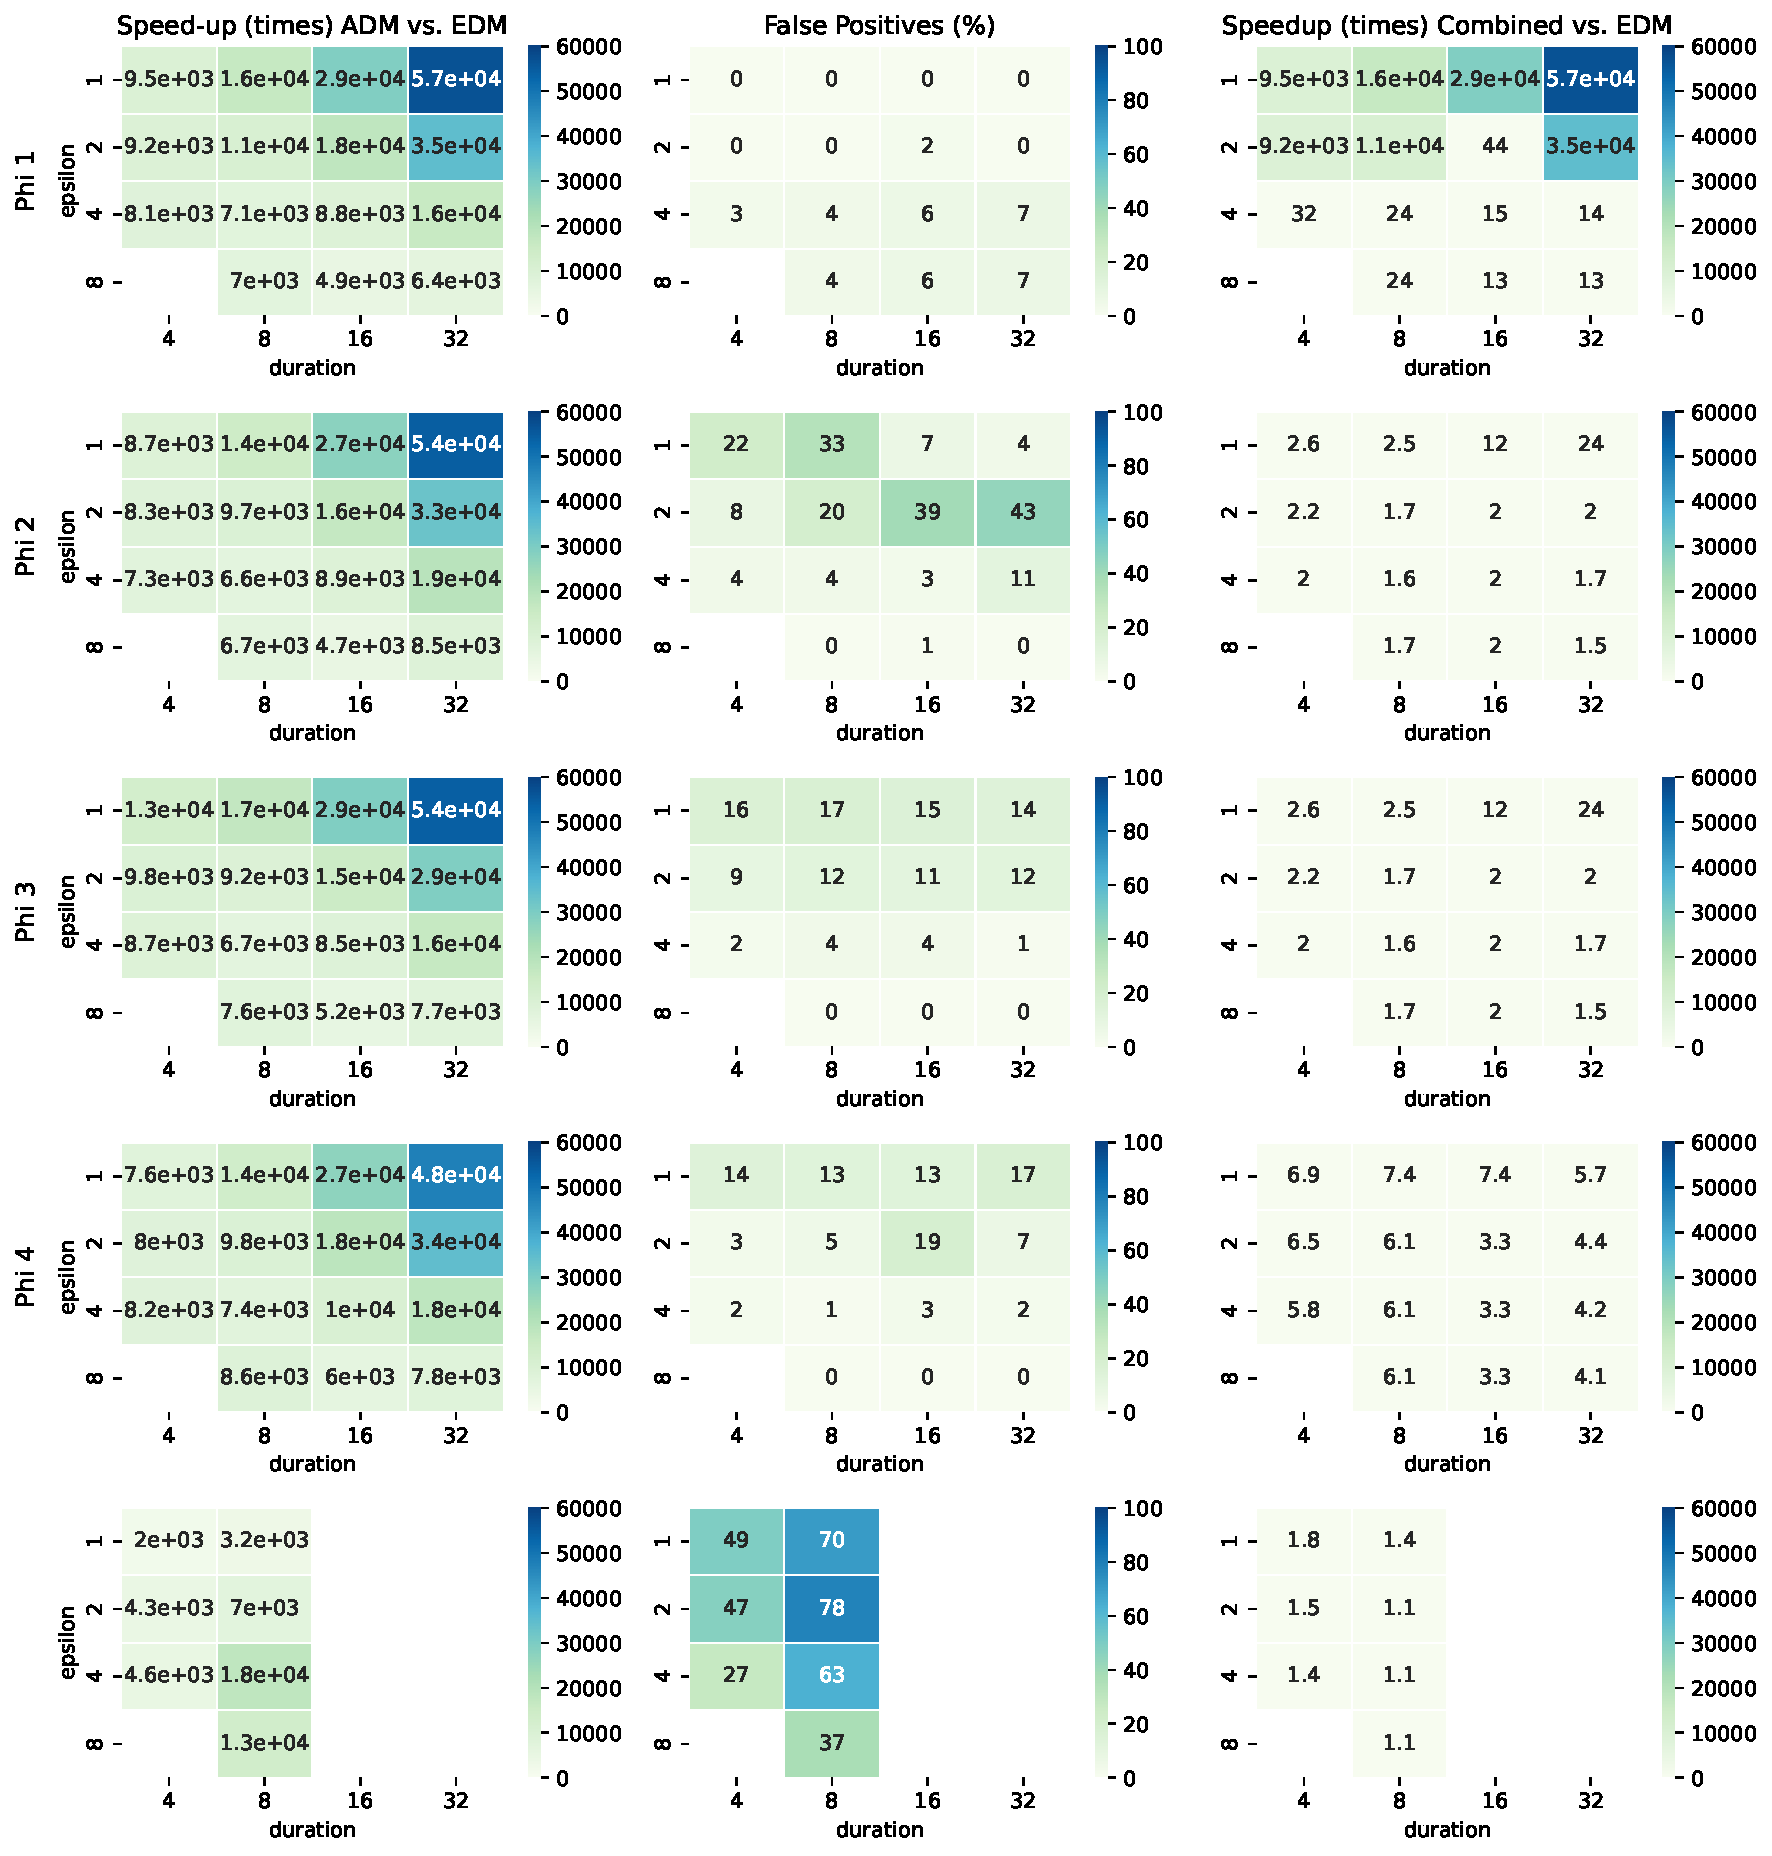
\includegraphics[width=\linewidth]{speedup}
\caption{The experimental results - monitoring of specifications $\varphi_{1}$ to $\varphi_{5}$ on distributed traces created by the RG.}
\label{fig:rgresults}
\end{center}
\end{figure}

We first observe that the approximate ADM approach consistently achieves computational speedups of \emph{several orders of magnitude} 
compared to the exact EDM approach. The absolute speedups range from several thousands to almost 60 thousand times, regardless of the considered specification, the duration $d$ of the trace, or the uncertainty $\epsilon$ bound. We see that the highest speedups are achieved for long signals with low uncertainty bounds. The price paid in terms of accuracy is highly dependendent on the type of specification and the uncertainty bounds. We can see that applying ADM is very accurate when monitoring the property 
$\varphi_1$ in which both the temporal and the combinatorial operators are conjunctive. On the other hand, having a combination of conjunctive and disjunctive operations (specifications $\varphi_{2}$, $\varphi_{3}$ and $\varphi_{4}$) increases the number of FPs.  Surprisingly, we see that in these cases the introduction of FPs is higher for lower values of $\epsilon$. This happens because that for higher values of $\epsilon$,  even the exact method gives many inconclusive verdicts. Finally, we see that adding real-time modalities to the temporal operators adds inacuracies and increases further the percentage of FPs. Finally, by observing the third column of Figure~\ref{fig:rgresults}, we can see that by combining EDM and ADM, we consistently get better performance than by using EDM only, even in cases where ADM introduces a high percentage of FPs.


\begin{figure}[htb]
	\begin{center}
		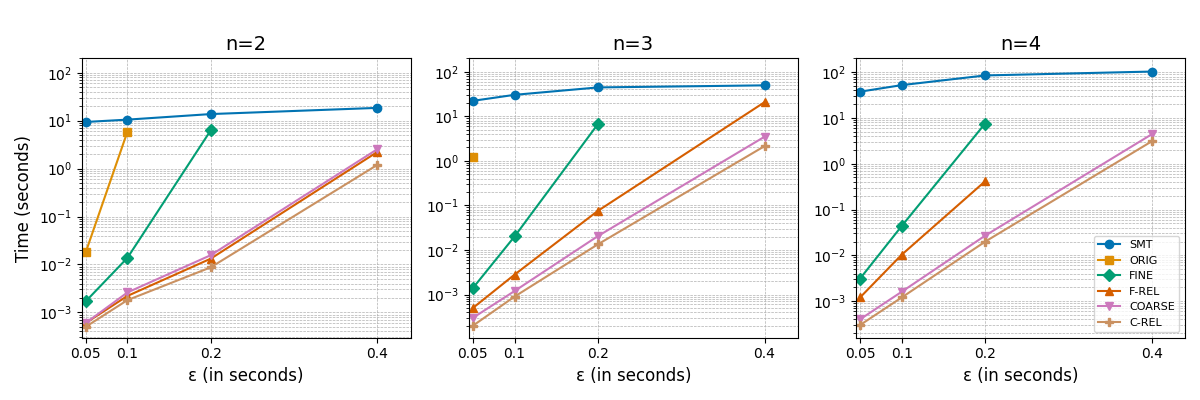
\includegraphics[width=\linewidth]{wtlin.png}
		\caption{Heat pump log-linear scale, out-of-time limit 120s}
	\end{center}
\end{figure}

\subsubsection{Heat Pump Discussion.}
Speedups increase with the number of signals \(n\) and decrease with the maximum clock skew \(\varepsilon\).
The \textsc{Coarse} method shows significant improvements over EDM, with up to a $104000\times$ speedup in the best-case (when \(n=4\) and \(\varepsilon=0.05\)) and an $8\times$ speedup in the worst-case (when \(n=2\) and \(\varepsilon=0.4\)).
Note that \(\varepsilon=0.4\) is near the realistic upper limit, indicating no scalability issues.
The decentralized \textsc{Coarse-Relative} method adds up to a $1.63\times$ speedup over \textsc{Coarse}.
Decentralization significantly benefits \textsc{Fine}, bringing it below the time-out limit with up to a $476\times$ speedup in non-time-out instances.
As expected, \textsc{Orig} does not perform well.
All methods produce the same verdict for the considered traces.

\begin{figure}[htb]
	\begin{center}
		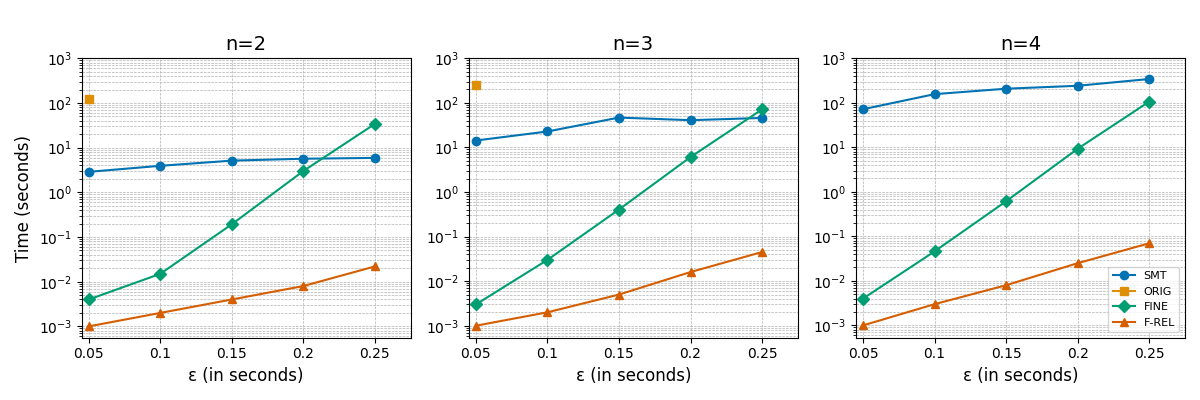
\includegraphics[width=\linewidth]{ms.png}
		\caption{Mutual separation log-linear scale, out-of-time limit 360s}
	\end{center}
\end{figure}

\subsubsection{Swarm of Drones Discussion.}
Similar to the previous case scenario, speedups in the mutual separation case increase with \(n\) and decrease with \(\varepsilon\).
The \textsc{Fine-Relative} method achieves about a $78000\times$ speedup in the best-case scenario (when \(n=4\) and \(\varepsilon=0.05\)) and a $23\times$ speedup in the worst-case (when \(n=2\) and \(\varepsilon=0.25\)).
The fine method performs slower than SMT in two cases where \(n\) is small and \(\varepsilon\) is large.
\ege{Does NTP guarantee a smaller $\varepsilon$ with fewer number of nodes?}
As in the previous case, \textsc{Orig} does not perform well.
Additionally, \textsc{Coarse} and \textsc{Coarse-Relative} are not applicable in this scenario because the arithmetic operations are not monotonic.
Again, all methods yield the same verdicts.

